\documentclass[12pt]{article}
\usepackage{hyperref}
\usepackage{graphicx}
\usepackage{mathtools}
\usepackage[margin=1in, paperwidth=8.5in, paperheight=11in]{geometry}
\begin{document}
\title{Istanbul Technical University- Spring 2017 \\ BLG527E Machine Learning \\ Homework 5}
\author{Ne\c{s}e Gune\c{s} \\ student number: 504161544 \\ 
	\href{mailto:gunesn17@itu.edu.tr}{gunesn17@itu.edu.tr} \and Omid Abdollahi Aghdam \\
student number: 504151520\\
\href{mailto:abdollahi15@itu.edu.tr}{abdollahi15@itu.edu.tr}\\
\href{mailto:abdollahi.omid@gmail.com}{abdollahi.omid@gmail.com}
}
\date{\today}
\maketitle
\newpage

\textbf{Q1)} We use svm classifier from sklearn library to train a model using precomputed kernel values and find alpha values. As we have look up from sklearn documentation \footnote{1.4.6.1.2. Using the Gram matrix: \\ http://scikit-learn.org/stable/modules/svm.html\#svm-kernels} \\ it is said that kernel values between all training vectors and the test vectors must be provided. However, we do not have kernel values for test data points. The provided kernel matrix  is for training data. We also submit code we used in the attachment.\\ \\
\textbf{Q2 a)} Observation sequence is $\{O_1 = a, O_2=a, O_3=b\}$, we calculate $P(O | A, B, \Pi)$ using forward variable. Th

\textbf{Initialization:}\\
We denote state 1 and 2 with $S_1, S_2$ respectively.
\begin{equation}
	\begin{aligned}
		\alpha_{t=1}(S_1) &= \pi_{S_1}b_{S_1}(a)\\
						&= 0.9 \times 0.1\\
						&=0.09 \\ \\
	\end{aligned}
\end{equation}

\begin{equation}
	\begin{aligned}
		\alpha_{t=1}(S_2) &= \pi_{S_2}b_{S_2}(a)\\
		&= 0.1 \times 0.9\\
		&=0.09 \\ \\
	\end{aligned}
\end{equation}

\textbf{Recursion:}\\
\begin{equation}
	\begin{aligned}
		\alpha_{t=2}(S_1) &= [ \Sigma_{i=1}^2 \alpha_{t=1}(i)a_{i1}]b_{S_1}(a)\\
		&= [0.09 \times 0.8 + 0.09 \times 0.2]0.1\\
		&= 0.009\\ \\
	\end{aligned}
\end{equation}

\begin{equation}
	\begin{aligned}
		\alpha_{t=2}(S_2) &= [ \Sigma_{i=1}^2 \alpha_{t=1}(i)a_{i2}]b_{S_2}(a)\\
		&= [0.09 \times 0.2 + 0.09 \times 0.8]0.9\\
		&= 0.081
	\end{aligned}
\end{equation}

\begin{equation}
	\begin{aligned}
		\alpha_{t=3}(S_1) &= [ \Sigma_{i=1}^2 \alpha_{t=2}(i)a_{i1}]b_{S_1}(b)\\
		&= [0.09 \times 0.8 + 0.81 \times 0.2]0.9\\
		&= 0.2106
	\end{aligned}
\end{equation}

\begin{equation}
	\begin{aligned}
		\alpha_{t=3}(S_2) &= [ \Sigma_{i=1}^2 \alpha_{t=2}(i)a_{i2}]b_{S_2}(b)\\
		&= [0.09 \times 0.2 + 0.81 \times 0.8]0.1\\
		&= 0.0666
	\end{aligned}
\end{equation}

\begin{equation}
	\begin{aligned}
		p(O | A, B, \pi) &= \Sigma_{i=1}^2 \alpha_T(i)\\
		&=\alpha_{t=3}(S_1) + \alpha_{t=3}(S_2)\\
		&= 0.0164 + 0.065\\
		&= 0.2772
	\end{aligned}
\end{equation}
\textbf{Q2 b)} 
We use the Viterbi algorithm to find the most probable state sequence given \\O = a, a, b.\\
\textbf{Initialization:}
\begin{equation}
	\begin{aligned}
		\delta_{t=1}(1) &= \pi_{1}b_{1}(a) \\
		& = 0.9 \times 0.1 \\
		& = 0.09 \\
		\delta_{t=1}(2) &= \pi_{2}b_{2}(a) \\
		& = 0.1 \times 0.9 \\
		& = 0.09 \\ \\
		\psi_{t=1}(1) &= 0 \\
		 \psi_{t=1}(2) &= 0 \\ 
	\end{aligned}
\end{equation}
\textbf{Recursion:}
\begin{equation}
	\begin{aligned}
		\delta_{t=2}(1) &= \underset{i}{max} \delta_{t=1}(i)a_{i1}.b_1(a) \\
		&= max(\delta_{t=1}(1)a_{11}.b_1(a), \delta_{t=1}(2)a_{21}.b_1(a)) \\
		&= max(0.09 \times 0.8 \times 0.1, 0.09 \times 0.2 \times 0.1) \\
		&= max(0.0072, 0.0018) \\
		&= 0.0072 \\ \\
		\delta_{t=2}(2) &= \underset{i}{max} \delta_{t=1}(i)a_{i2}.b_2(a) \\
		&= max(\delta_{t=1}(1)a_{12}.b_2(a), \delta_{t=1}(2)a_{22}.b_2(a)) \\
		&= max(0.09 \times 0.2 \times 0.9, 0.09 \times 0.8 \times 0.9) \\
		&= max(0.0162, 0.0648) \\
		&= 0.0648 \\ \\
		\delta_{t=3}(1) &= \underset{i}{max} \delta_{t=2}(i)a_{i1}.b_1(b) \\
		&= max(\delta_{t=2}(1)a_{11}.b_1(b), \delta_{t=2}(2)a_{21}.b_1(b)) \\
		&= max(0.0072 \times 0.8 \times 0.9, 0.0648 \times 0.2 \times 0.9) \\
		&= max(0.005184, 0.011664) \\
		&= 0.011664 \\ \\
		\delta_{t=3}(2) &= \underset{i}{max} \delta_{t=2}(i)a_{i2}.b_2(b) \\
		&= max(\delta_{t=2}(1)a_{12}.b_2(b), \delta_{t=2}(2)a_{22}.b_2(b)) \\
		&= max(0.0072 \times 0.2 \times 0.1, 0.0648 \times 0.8 \times 0.1) \\
		&= max(0.000144, 0.005184) \\
		&= 0.005184 \\ \\
	\end{aligned}
\end{equation}
\begin{equation}
	\begin{aligned}
		\psi_{t=2}(1)&=\underset{i}{argmax}(\delta_{t=1}(i)a_{i1}) \\
		&=argmax(\delta_{t=1}(1)a_{11}, \delta_{t=1}(2)a_{21}) \\
		&=argmax(0.09 \times 0.8, 0.9 \times 0.2) \\
		&=argmax(0.072, 0.018) \\
		&=S_1 \\ \\
		\psi_{t=2}(2)&=\underset{i}{argmax}(\delta_{t=1}(i)a_{i2}) \\
		&=argmax(\delta_{t=1}(1)a_{12}, \delta_{t=1}(2)a_{22}) \\
		&=argmax(0.09 \times 0.2, 0.09 \times 0.8) \\
		&=argmax(0.018, 0.072) \\
		&=S_2 \\ \\
		\psi_{t=3}(1)&=\underset{i}{argmax}(\delta_{t=2}(i)a_{i1}) \\
		&=argmax(\delta_{t=2}(1)a_{11}, \delta_{t=2}(2)a_{21}) \\
		&=argmax(0.0072 \times 0.8, 0.0648 \times 0.2) \\
		&=argmax(0.00576, 0.01296) \\
		&=S_2 \\ \\
		\psi_{t=3}(2)&=\underset{i}{argmax}(\delta_{t=2}(i)a_{i2}) \\
		&=argmax(\delta_{t=2}(1)a_{12}, \delta_{t=2}(2)a_{22}) \\
		&=argmax(0.0072 \times 0.2, 0.0648 \times 0.8) \\
		&=argmax(0.00144, 0.05184) \\
		&=S_2 \\ \\
	\end{aligned}
\end{equation}
\newpage
\textbf{Termination:}
\begin{equation}
	\begin{aligned}
		p^*&=\underset{i}{max}(\delta_{t=3}(i)) \\
		&=max(0.011664, 0.005184) \\
		&=0.011664 \\ \\
		q_{t=3}^*&=\underset{i}{argmax}(\delta_{t=3}(i)) \\
		&=argmax(0.011664, 0.005184) \\
		&=S_1 \\ \\
	\end{aligned}
\end{equation}
\textbf{Path:}
\begin{equation}
	\begin{aligned}
		q_{t=2}^*&=\psi_{t=3}(q_{t=3}^*) \\
		&=\psi_{t=3}(S_1) \\
		&=S_2 \\ \\
		q_{t=1}^*&=\psi_{t=2}(q_{t=2}^*) \\
		&=\psi_{t=2}(S_2) \\
		&=S_2 \\ \\
	\end{aligned}
\end{equation}
Using the Viterbi algorithm the most probable state sequence given O is $Q=S_{2}S_{2}S_{1}$.\newpage
\textbf{Q3 )} 
We have the following information:
\begin{equation}
	\begin{aligned}
		P(X_i | X_{i-1}) = 0.8 \\
		P(\sim X_i | X_{i-1}) = 0.2 \\
		P(X_i | \sim X_{i-1}) = 0.1 \\
		P(\sim X_i | \sim X_{i-1}) = 0.9 \\
		P(X_1) = 0.2
	\end{aligned}
\end{equation}

\begin{equation}
	\begin{aligned}
		P(X_3 | X_1, \sim X_4) = \alpha \pi (X_3) \lambda (X_3)
	\end{aligned}
\end{equation}

\begin{equation}
	\begin{aligned}
		\pi (X_3) &= \Sigma_{X_2} P(X_3 | X_2) \pi(X_2)\\
		&=P(X_3 | X_2)\pi(X_2) + P(X_3 | \sim X_2)\pi(\sim X_2)\\
		&=P(X_3 | X_2)P(X_2 | X_1)P(X_1) \\
		&+ P(X_3 | \sim X_2)P(\sim X_2 | X_1)P(X_1) \\
		&= 0.8 \times 0.8 \times 0.2 + 0.1 \times 0.2 \times 0.2 \\
		&= 0.132
	\end{aligned}
\end{equation}

\begin{equation}
	\begin{aligned}
		\lambda (X_3) &= P(\sim X_4 | X_3)\lambda(\sim X_4) \\
		&= 0.2 \\ \\
	\end{aligned}
\end{equation}
Now we have:
\begin{equation}
	\begin{aligned}
		P(X_3 | X_1, \sim X_4) &=0.132 \times 0.2 \alpha \\
		&= 0.0264 \alpha
	\end{aligned}
\end{equation}
In order to find the $\alpha$ we use the following summation.
\begin{equation}
		P(X_3 | X_1, \sim X_4) + 	P(\sim X_3 | X_1, \sim X_4) = 1
\end{equation}
\begin{equation}
	\begin{aligned}
		P(\sim X_3 | X_1, \sim X_4) = \alpha \pi (\sim X_3) \lambda (\sim X_3)
	\end{aligned}
\end{equation}
\begin{equation}
	\begin{aligned}
		\pi (\sim X_3) &= \Sigma_{X_2} P(\sim X_3 | X_2) \pi(X_2)\\
		&=P(\sim X_3 | X_2)\pi(X_2) + P(\sim X_3 | \sim X_2)\pi(\sim X_2)\\
		&=P(\sim X_3 | X_2)P(X_2 | X_1)P(X_1) \\
		&+ P(\sim X_3 | \sim X_2)P(\sim X_2 | X_1)P(X_1) \\
		&= 0.2 \times 0.8 \times 0.2 + 0.9 \times 0.2 \times 0.2 \\
		&= 0.068
	\end{aligned}
\end{equation}

\begin{equation}
	\begin{aligned}
		\lambda (\sim X_3) &= P(\sim X_4 | \sim X_3)\lambda(\sim X_4) \\
		&= 0.9 \\ \\
		P(\sim X_3 | X_1, \sim X_4) &=0.068 \times 0.9 \alpha \\
		&= 0.0612 \alpha
	\end{aligned}
\end{equation}
We replace the results in equation 18 to find the $\alpha$.
\begin{equation}
	\begin{aligned}
		0.0264 \alpha + 0.0612 \alpha &= 1 \\
		0.0876 \alpha &= 1 \\
		\alpha &= 11.415
	\end{aligned}
\end{equation}
\begin{equation}
	\begin{aligned}
		P(X_3 | X_1, \sim X_4) &=0.132 \times 0.2 \alpha \\
		&= 0.0264 \times 11.415 \\
		&=0.301559
	\end{aligned}
\end{equation}
\textbf{Q4 a)}
We use the K-Fold paired cross-validated t-Test to solve this. If the two classifiers have the same error rate we they must have the same error rate mean.Thus, the difference of their error rate mean is zero. We calculate their error difference as show in the column 3 of Table \ref{error}

\begin{table}[h!]
	\centering
	\caption{Error rate of two classifiers and their difference.}
	\label{error}
	\begin{tabular}{|l|l|l|}
		\hline
		MLP  & KNN  & Pi    \\ \hline
		0.00 & 0.00 & 0.00  \\ \hline
		0.00 & 0.07 & -0.07 \\ \hline
		0.00 & 0.00 & 0.00  \\ \hline
		0.07 & 0.07 & 0.00  \\ \hline
		0.13 & 0.13 & 0.00  \\ \hline
		0.00 & 0.00 & 0.00  \\ \hline
		0.13 & 0.07 & 0.06  \\ \hline
		0.00 & 0.00 & 0.00  \\ \hline
		0.00 & 0.00 & 0.00  \\ \hline
		0.00 & 0.00 & 0.00  \\ \hline
	\end{tabular}
\end{table}

We use the null hypothesis to accept or reject that the error rate mean is zero.
\begin{equation}
	\begin{aligned}
		H_0 : \mu = 0 \\
		H_1 : \mu \neq 0 \\
	\end{aligned}
\end{equation}
We use the following equations to calculate mean and variance of error rates difference.
\begin{equation}
	\begin{aligned}
		m = \frac{\Sigma_{i=1}^K p_i}{K} \\
		S^2 = \frac{\Sigma_{i=1}^K (p_i - m)^2}{K-1} \\
		m = -0.001 \\
		S^2 = 0.000943 \\
	\end{aligned}
\end{equation}
Under the null hypothesis that $\mu = 0$, we use the following t-Distributed statistic with K-1 degree of freedom. 
\begin{equation}
	\begin{aligned}
		\frac{\sqrt{K} (m)}{\sqrt{S^2}} \sim t_{K-1} \\
		\frac{\sqrt{10} (-0.001)}{\sqrt{0.000943}} \sim t_{K-1} \\
		-0.10298 \sim t_{K-1}
	\end{aligned}
\end{equation}
If K-Fold cv paired t-Test reject the hypotheses that Two classifiers have the same error rates at significance level of $\alpha=0.05$ if the value (-0.10298) is outside the $(-t_{0.025,9}, t_{0.025,9})$ which we look up from t-Table and the resulted interval is (-2.26216, 2.26216). As -0.10298 is inside the interval so we \textbf{accept the hypothesis.} Thus, the two classifiers have the same error rates.\\ \\
\textbf{Q4 b)} We use the following null hypothesis and to accept or reject that the classification algorithms have the same expected error rates as significance level $\alpha=0.05$.
\begin{equation}
	\begin{aligned}
		H_0 : \mu_{MLP} = \mu_{KNN} = \mu_{NB} \\
		H_1 : \mu_{r} \neq \mu_{s}, \hspace{0.2cm} \text{for at least one pair (r, s)} \\
	\end{aligned}
\end{equation}
We calculate the mean of error rates for each class.
\begin{equation}
	\begin{aligned}
		m_{MLP} &= \Sigma_{i=1}^{10} \frac{X_{iMLP}}{10} \\
		&=0.033 \\
		m_{KNN} &= \Sigma_{i=1}^{10} \frac{X_{iKNN}}{10} \\
		&=0.034 \\	
		m_{KNN} &= \Sigma_{i=1}^{10} \frac{X_{iNB}}{10} \\
		&=0.048 \\		
	\end{aligned}
\end{equation}
Now we calculate the mean and variance of errors for all classifiers.
\begin{equation}
	\begin{aligned}
		m &= \Sigma_{j=1}^{3} \frac{m_j}{L} \\
		&=\frac{m_{MLP}+m_{KNN}+m_{NB}}{3}\\
		m &= 0.0383 \\
		S^2 &= \Sigma_{j=1}^{3} \frac{(m_j - m)^2}{L - 1} \\
		&=7.0335 \times 10^{-5} \\		
	\end{aligned}
\end{equation}
Now we calculate between groups sum of squares.
\begin{equation}
	\begin{aligned}
		SS_b &= \Sigma_{j=1}^{3} (m_j - m)^2 \\
		&=0.001407	
	\end{aligned}
\end{equation}
We also need within group sum of squares.
\begin{equation}
	\begin{aligned}
		SS_w &= \Sigma_{j=1}^{3}\Sigma_{i=1}^{10} (X_{ij} - m_j)^2 \\
		&=7(-0.033)^2 + 2(0.13-0.033)^2 +(0.07-0.033)^2 \\
		&=6(-0.034)^2 + 3(0.07-0.034)^2 +(0.13-0.034)^2	\\
		&=5(0.07-0.048)^2 + 4(-0.048)^2 +(0.13-0.048)^2	\\
		&=0.06621
	\end{aligned}
\end{equation}
Using the calculated sum of squares we calculate $F_0$ value and look up its value from F distribution table.
\begin{equation}
\begin{aligned}
	F_0 &= \frac{SS_b /(L-1)}{SS_w/(L(K-1))} \\
		&=\frac{0.001407/2}{0.06621/27} \\
		&=0.28688
	\end{aligned}
\end{equation}
If $F_0$ is greater than $F_{2,27}$ at $\alpha=0.05$ significance level we reject the hypothesis. We look up F Table and $F_{2,27} = 3.35$. \textbf{We accept} the hypothesis, because $F_0$ is not greater than $F_{2,27}$. So $error_{MLP} = error_{KNN} = error_{NB}$.
\newpage
\textbf{Attachments:}
We create a csv file for dataset as follow and then use the following code.\newline
1.6715,2.0347,1,1.00,0.22,0.36,0.41,0.23,0.15,0.04,0.03,0.06,0.02\\
-0.2075,1.7269,1,0.22,1.00,0.17,0.11,0.16,0.37,0.10,0.06,0.19,0.03\\
1.7172,0.6966,1,0.36,0.17,1.00,0.46,0.78,0.23,0.06,0.05,0.07,0.02\\
2.6302,1.2939,1,0.41,0.11,0.46,1.00,0.29,0.11,0.04,0.03,0.05,0.02\\
1.4889,0.2127,1,0.23,0.16,0.78,0.29,1.00,0.28,0.07,0.06,0.08,0.03\\
-0.1116,0.4384,-1,0.15,0.37,0.23,0.11,0.28,1.00,0.16,0.10,0.26,0.04\\
-2.1471,-0.6748,-1,0.04,0.10,0.06,0.04,0.07,0.16,1.00,0.46,0.45,0.12\\
-2.0689,-1.7549,-1,0.03,0.06,0.05,0.03,0.06,0.10,0.46,1.00,0.18,0.18\\
-1.8095,0.3703,-1,0.06,0.19,0.07,0.05,0.08,0.26,0.45,0.18,1.00,0.07\\
-3.9443,-2.7115,-1,0.02,0.03,0.02,0.02,0.03,0.04,0.12,0.18,0.07,1.00\\


\begin{figure}[h!] 
	\begin{center}
		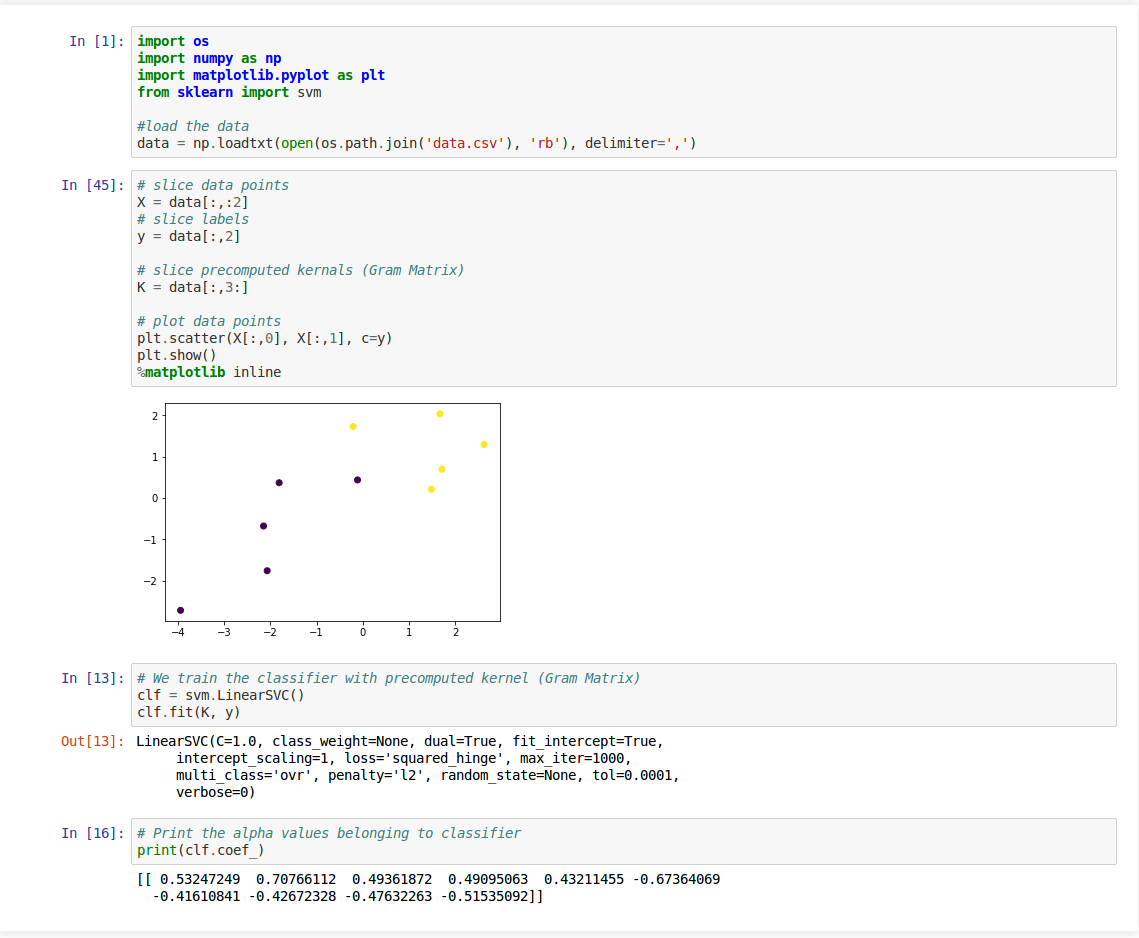
\includegraphics[width=\textwidth]{hw.png}
		\label{fig:test}
	\end{center}
\end{figure}  
\end{document}